\section{24 H 挂机功能}

本集成工具通过实时确定游戏内状态,执行相应的挂机动作。
因此,本集成工具完美支持挂机掉线后重连以及因为各种原因离开房间(如房间长时间未开始游戏导致关闭、被强制踢出等)后重新创建地狱围栏房间继续挂机。
挂机功能共分为两种:单人单件武器挂机(1 号功能)挂机及野房随机武器挂机(2 号功能)。
1 号功能可以搭配配件武器使用。2 号功能可以搭配特殊武器使用(如圣翼皓印)。
本集成工具支持选择 T 阵营或 CT 阵营角色。通关失败自动回合重置。
除了灾变挂机外,还可用于梦幻之星等荣誉图挂机。

使用挂机功能前,需要自行配置好游戏内各按钮的坐标位置以及挂机使用的武器列表。

\subsection{前提条件}

TCGame \textbf{必须} 设置为自动登录,并在本集成工具启动后 \textbf{必须} 保证登录信息尚未失效,否则将无法使用断线重连功能。

\textbf{建议}将游戏设置为窗口化运行。

本工具在游戏启动时会自动去除窗口的标题栏,并将窗口移动到屏幕正中央位置,防止因预料之外的窗口位置移动导致配置好的坐标信息失效。
因此,\textbf{强烈建议}本集成工具搭配 GamingTool 工具在将游戏窗口标题栏去掉并居中(GamingTool 的无边框窗口化功能)后再使用本集成工具 5 号功能确定游戏内各按钮坐标,
以保证坐标正确无误,并 \textbf{建议}在挂机时使用 GamingTool 隐藏游戏任务栏。

\href{https://gitee.com/silver1867/gaming-tool}{GamingTool 工具链接}

\subsection{配置 24 H 挂机功能}

\subsubsection{配置}

打开 lua 目录下的 \lstinline{Setting.lua} 文件,视情况更改如下字段(所有的坐标均通过模式 5 坐标定位功能确定)。

\lstinline{TIME_ZONE} 操作系统时区,东半球为正数,西半球为负数。例如,中国处于东八区(UTC+08:00),则应将其设置为 8(默认配置)。

\begin{figure}[H]
    \Centering
    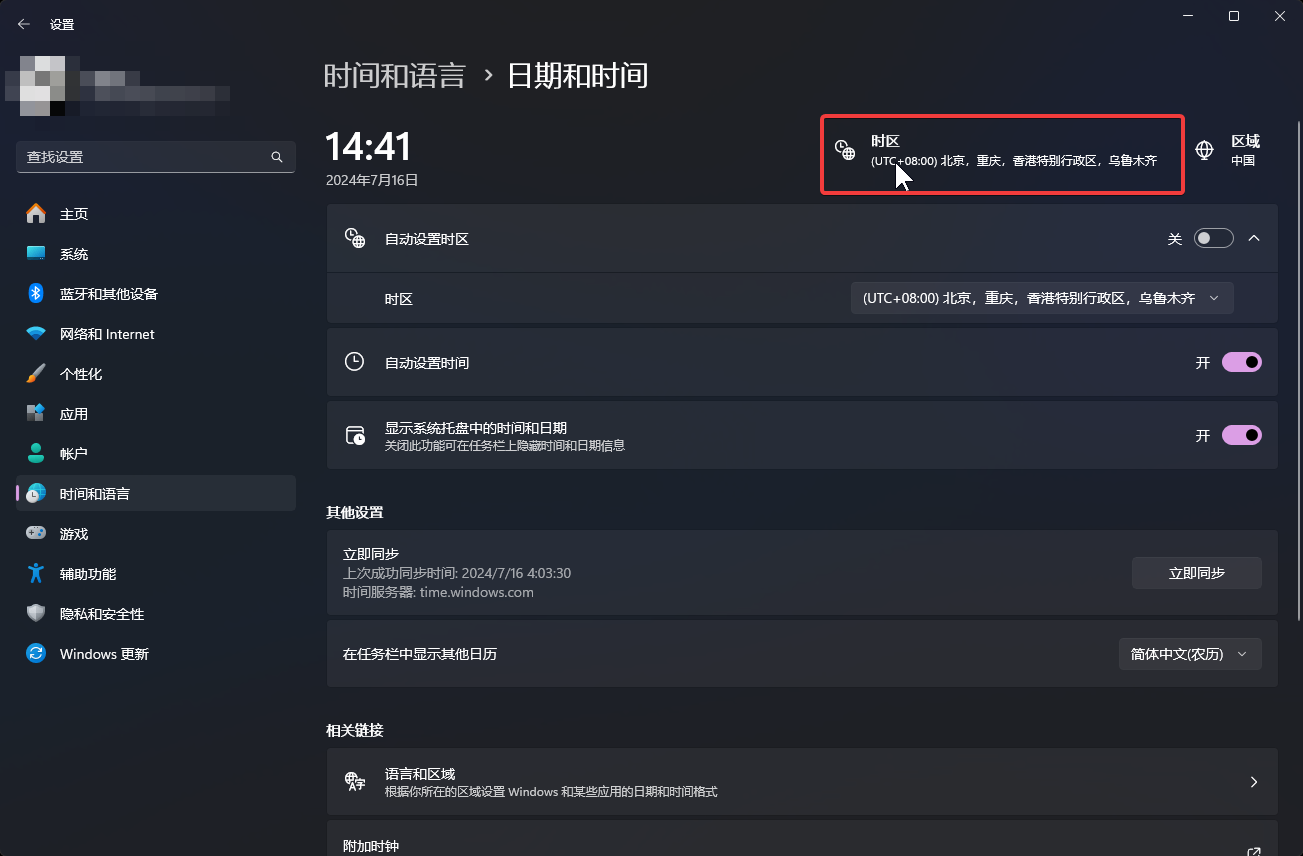
\includegraphics[width=\textwidth]{docs/assets/timezone.png}
    \caption{操作系统时区}
\end{figure}

\lstinline{HALL_ROOM_LIST_X}、\lstinline{ROOM_LIST_Y}:大厅房间列表选框的坐标。

\begin{figure}[H]
    \Centering
    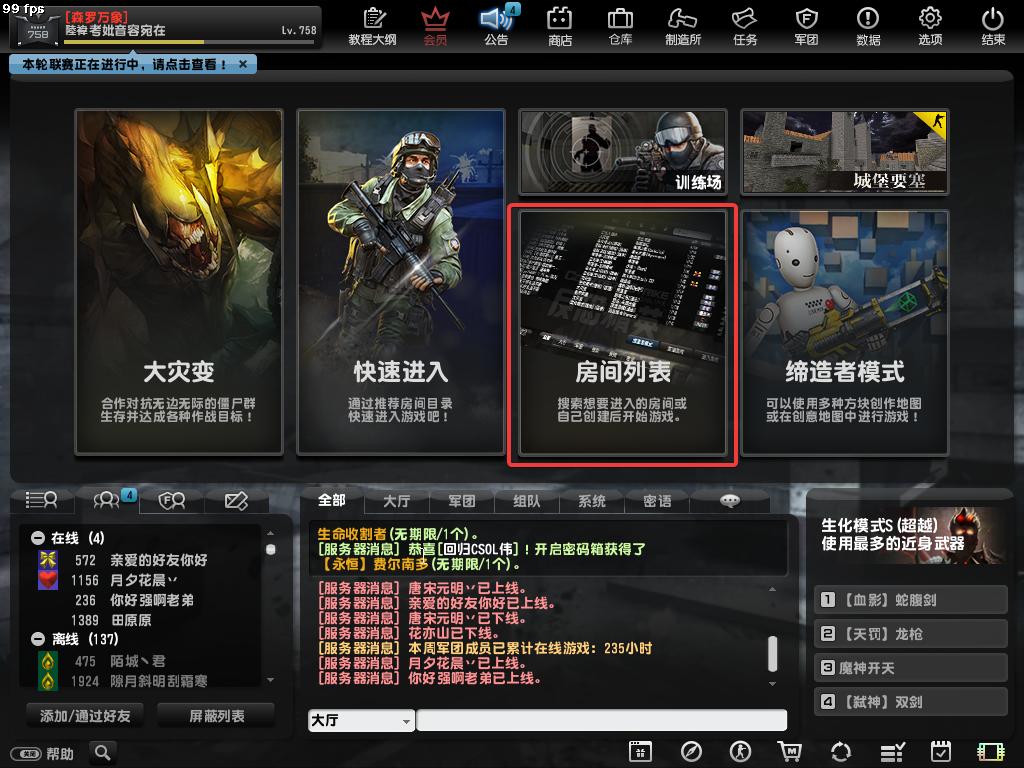
\includegraphics[width=\textwidth]{docs/assets/room_list.png}
    \caption{房间列表按钮}
\end{figure}

\lstinline{HALL_CREATE_ROOM_X}、\lstinline{HALL_CREATE_ROOM_Y}:大厅中的“新建房间”按钮坐标。

\begin{figure}[H]
    \Centering
    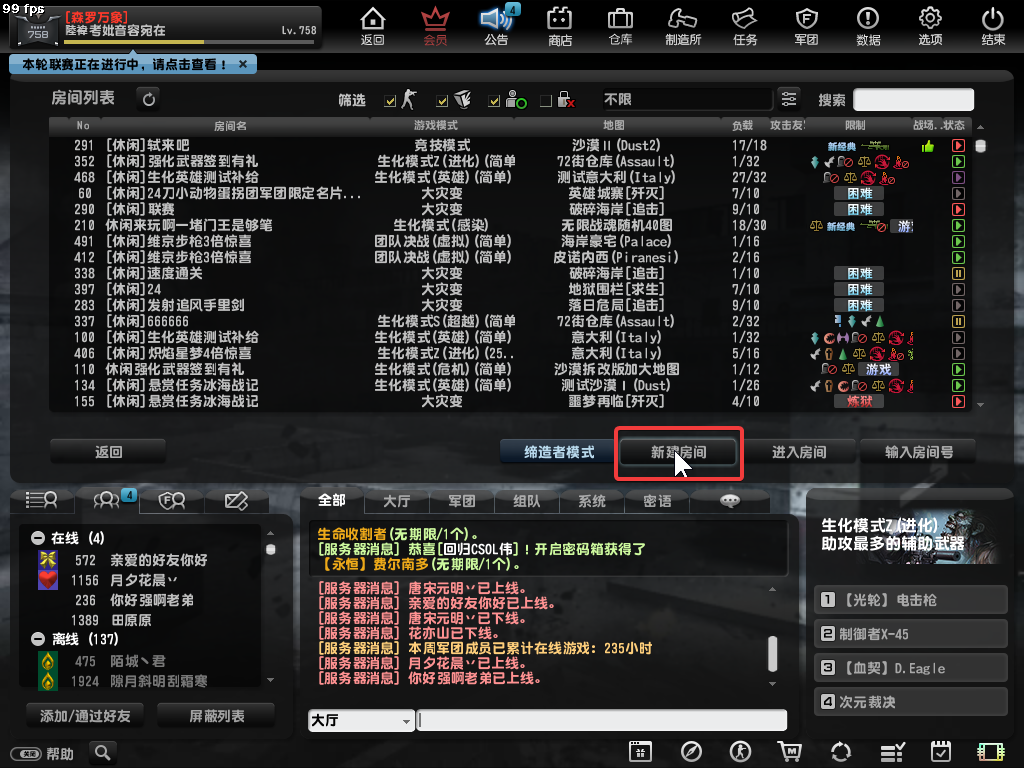
\includegraphics[width=\textwidth]{docs/assets/create_room_0}
    \caption{大厅中的“新建房间”按钮}
\end{figure}

\lstinline{HALL_BACK_X}、\lstinline{HALL_BACK_Y}:大厅房间列表界面中的“返回”按钮坐标。

\begin{figure}[H]
    \Centering
    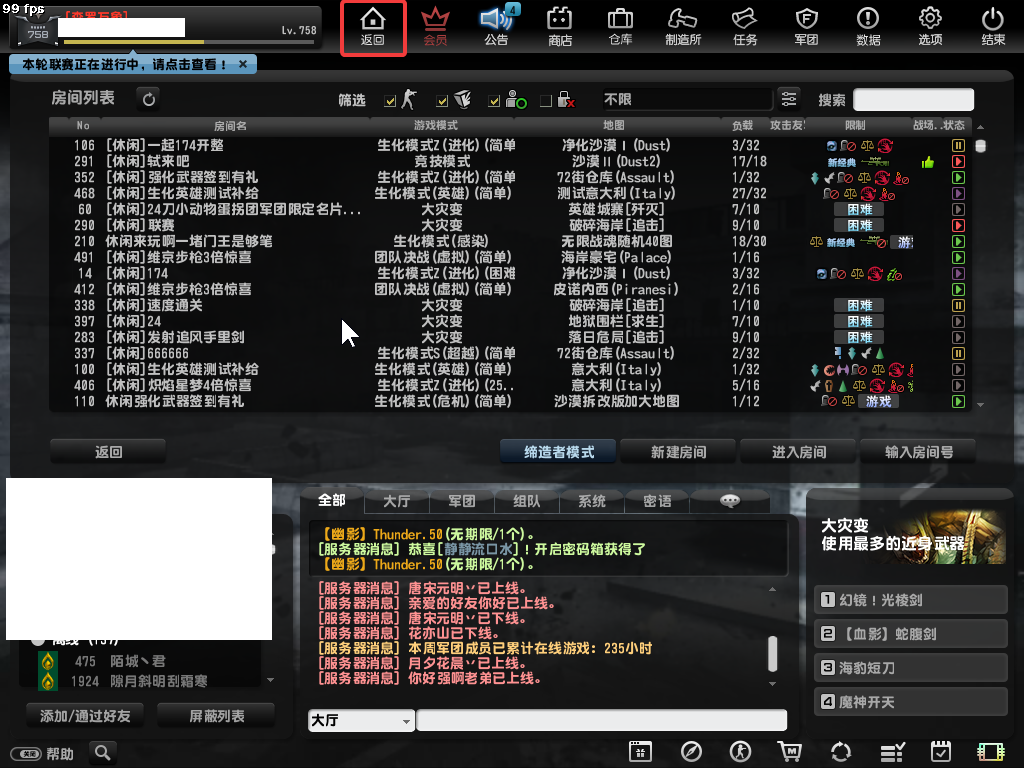
\includegraphics[width=\textwidth]{docs/assets/hall_back.png}
    \caption{大厅房间列表界面中的“返回”按钮}
\end{figure}

\lstinline{GAME_MODE_X}、\lstinline{GAME_MODE_Y}:点击大厅房间列表界面的“创建游戏”按钮后,弹出窗口中的“游戏模式”选框坐标。

\begin{figure}[H]
    \Centering
    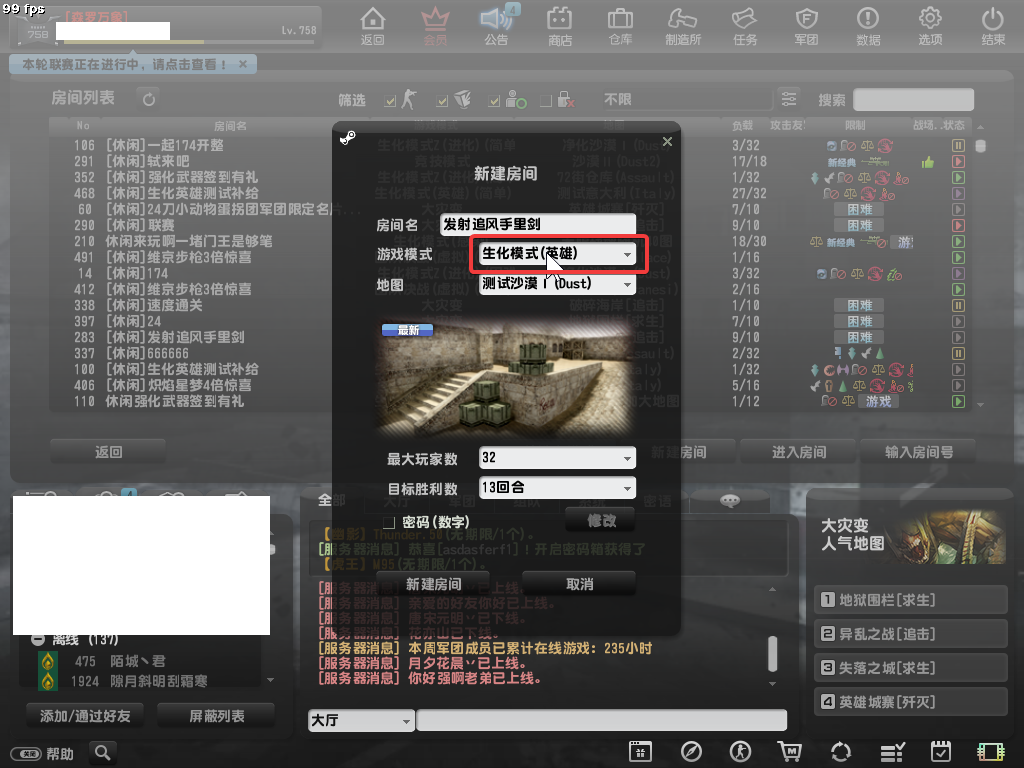
\includegraphics[width=\textwidth]{docs/assets/game_mode.png}
    \caption{“游戏模式”选框}
\end{figure}

\lstinline{ZOMBIE_SECNARIO_MODE_X}、\lstinline{ZOMBIE_SCENARIO_MODE_Y}:“大灾变”模式选框。

\begin{figure}[H]
    \Centering
    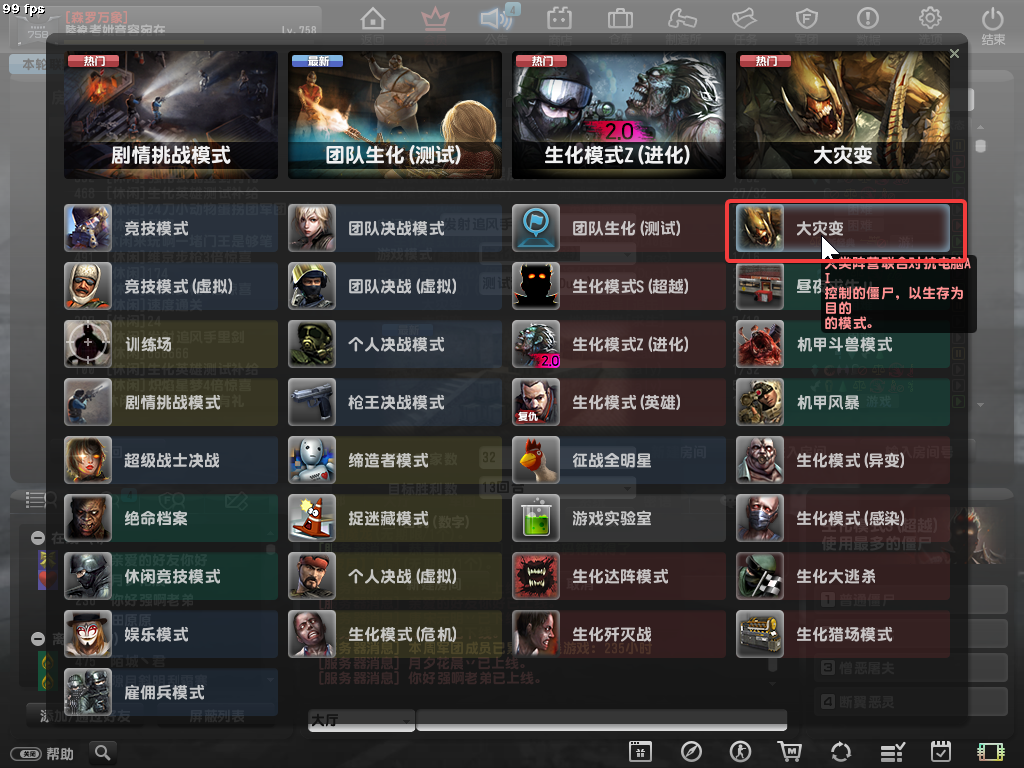
\includegraphics[width=\textwidth]{docs/assets/zombie_scenario.png}
    \caption{“大灾变”模式}
\end{figure}

\lstinline{MAP_CHOOSE_LEFT_SCROLL_X}、\lstinline{MAP_CHOOSE_LEFT_SCROLL_Y}:地图选择界面中的向左滚动按钮。

\begin{figure}[H]
    \Centering
    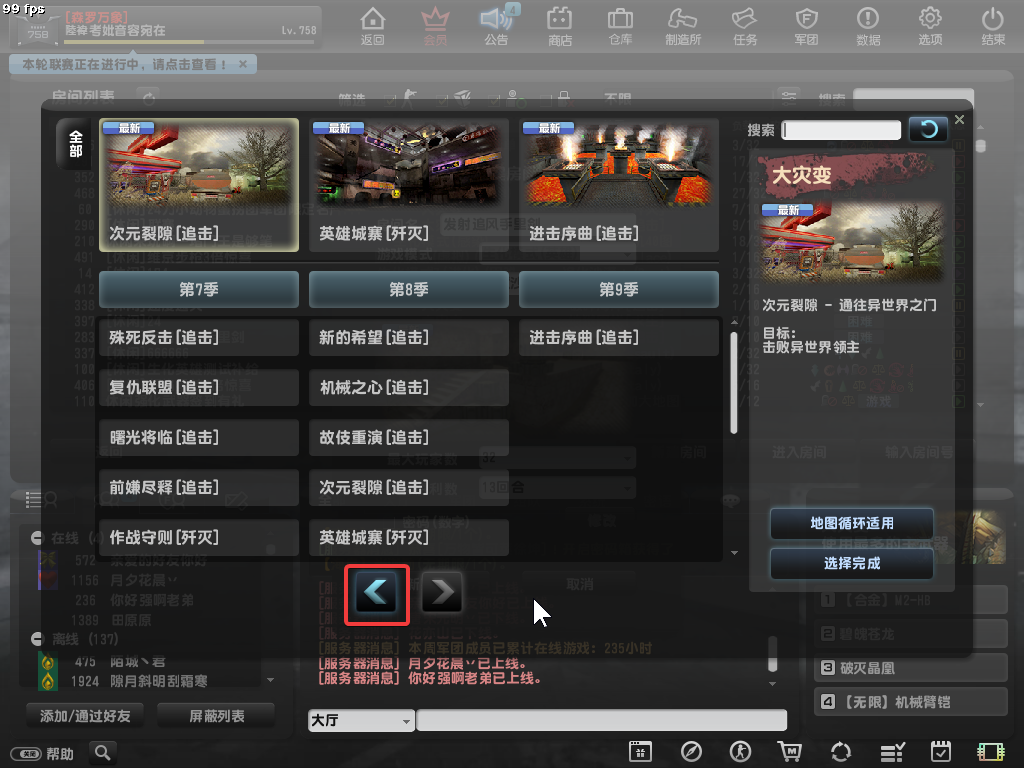
\includegraphics[width=\textwidth]{docs/assets/left_scroll.png}
    \caption{向左滚动按钮}
\end{figure}

\lstinline{MAP_TRAP_X}、\lstinline{MAP_TRAP_Y}:“地狱围栏”地图按钮坐标。

\begin{figure}[H]
    \Centering
    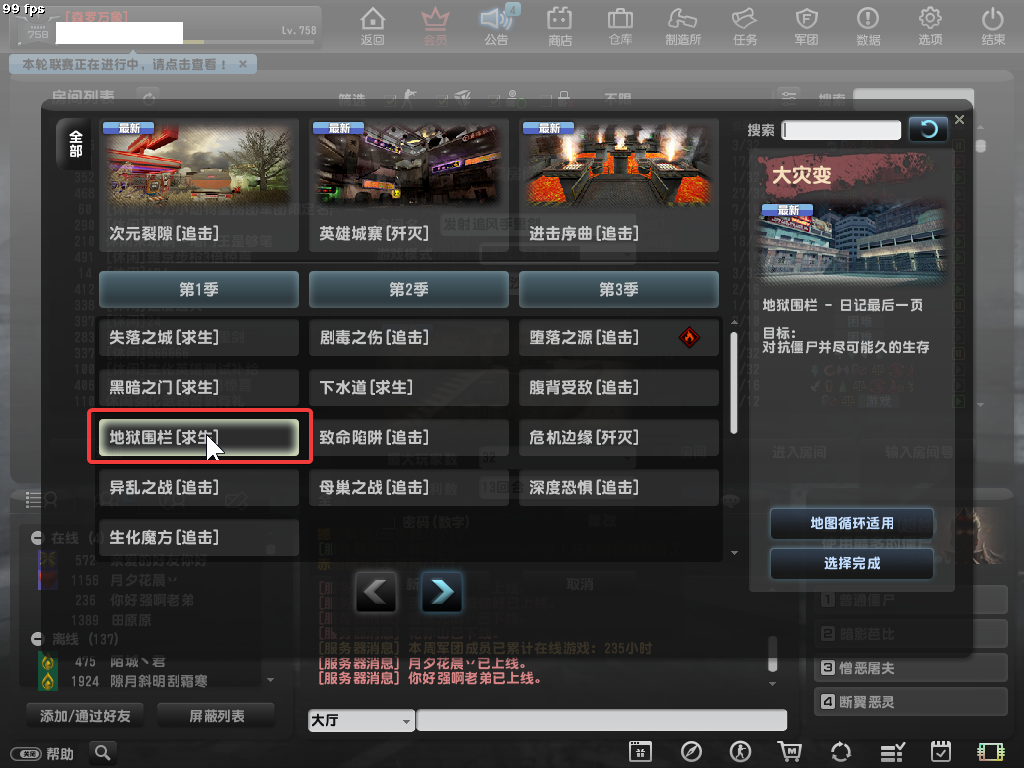
\includegraphics[width=\textwidth]{docs/assets/map_trap.png}
    \caption{“地狱围栏”地图}
\end{figure}

\lstinline{FINISH_CHOOSE_X}、\lstinline{FINISH_CHOOSE_Y}:“选择完成”按钮坐标。

\begin{figure}[H]
    \Centering
    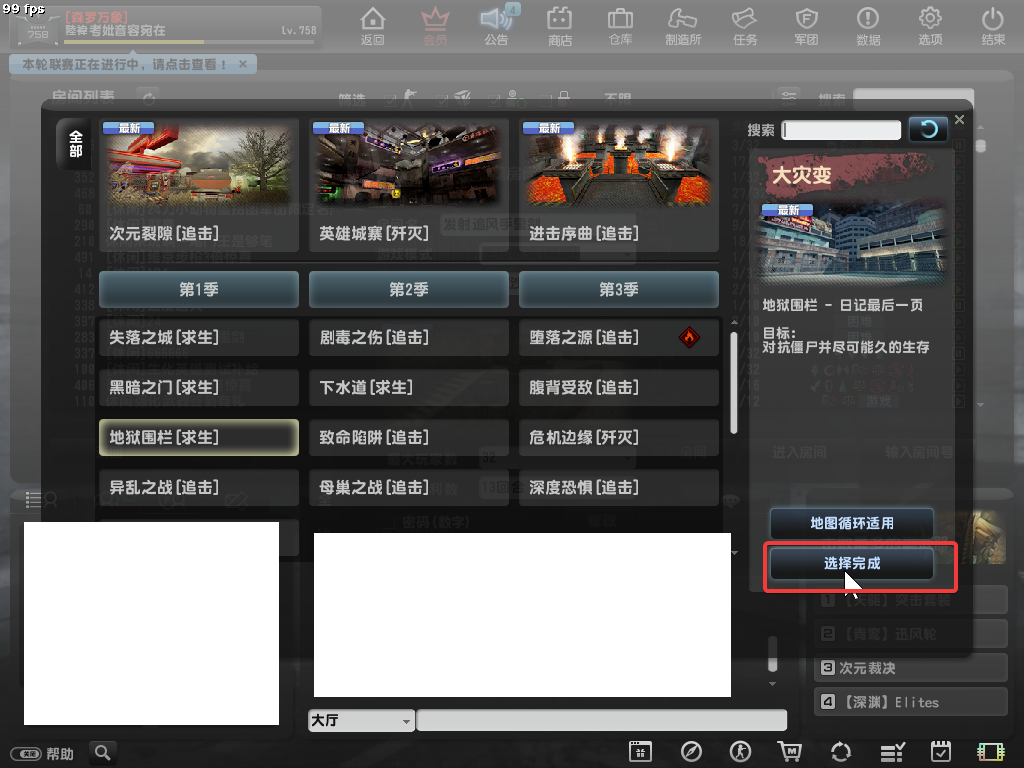
\includegraphics[width=\textwidth]{docs/assets/finish_choose.png}
    \caption{“选择完成”按钮}
\end{figure}

\lstinline{GAME_DIFFICULTY_X}、\lstinline{GAME_DIFFICULTY_Y}:“游戏难度”选框坐标。

\begin{figure}[H]
    \Centering
    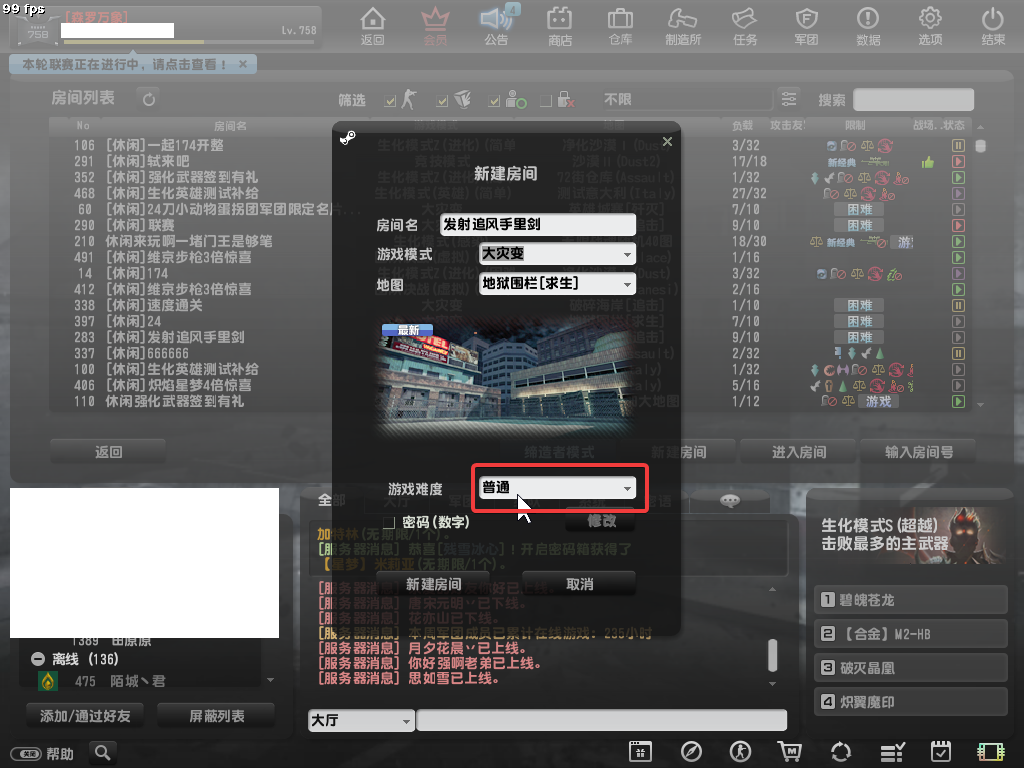
\includegraphics[width=\textwidth]{docs/assets/choose_difficulty.png}
    \caption{“游戏难度”按钮}
\end{figure}

\lstinline{GAME_DIFFICULTY_OPTION_X}、\lstinline{GAME_DIFFICULTY_OPTION_Y}:游戏难度选项坐标,建议设置为“困难”。

\begin{figure}[H]
    \Centering
    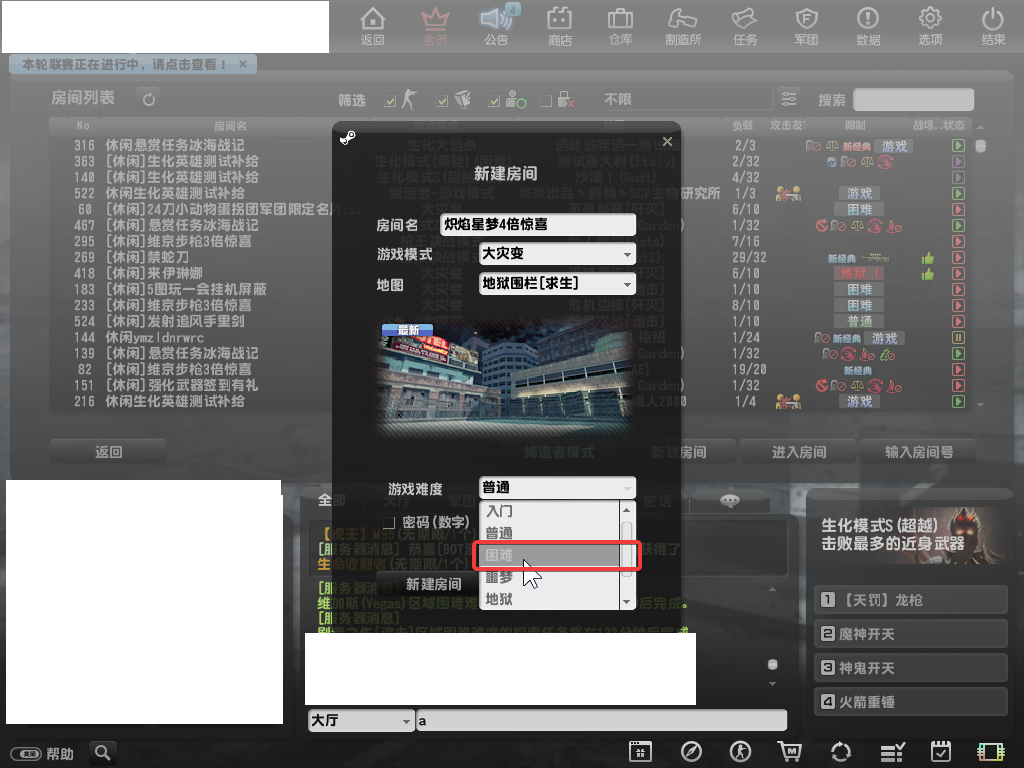
\includegraphics[width=\textwidth]{docs/assets/difficulty_option.png}
    \caption{游戏难度选项}
\end{figure}

\lstinline{CREATE_ROOM_X}、\lstinline{CREATE_ROOM_Y}:“新建房间”按钮坐标。

\begin{figure}[H]
    \Centering
    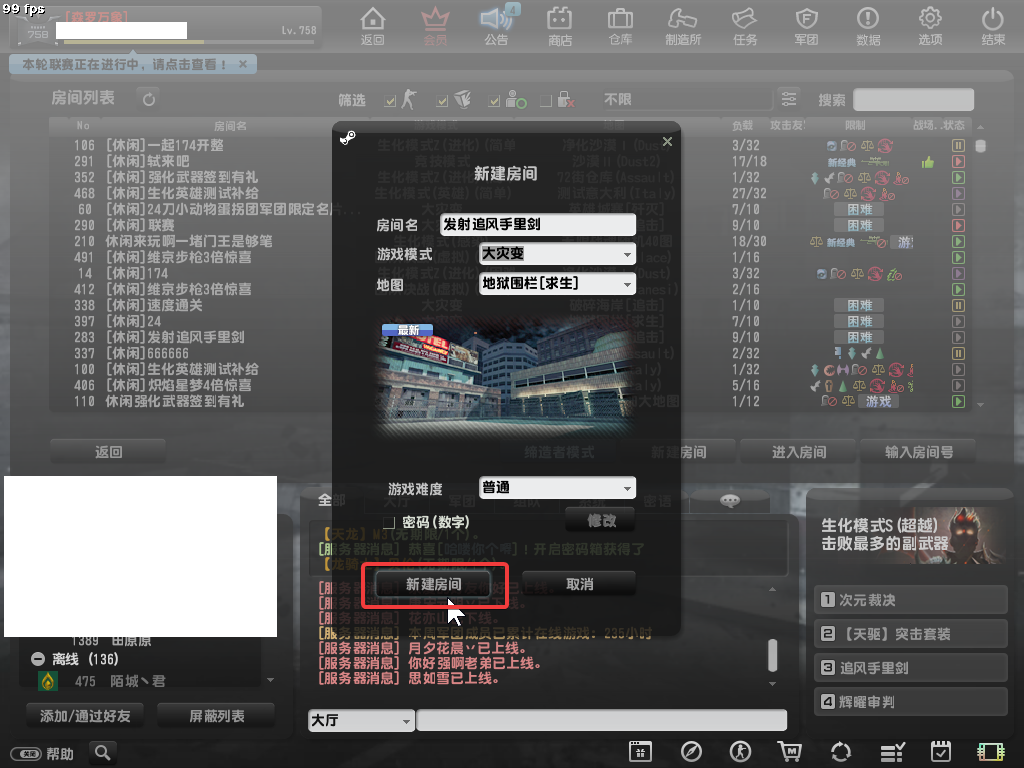
\includegraphics[width=\textwidth]{docs/assets/create_room_1.png}
    \caption{“新建房间”按钮}
\end{figure}

\lstinline{ROOM_GAME_START_X}、\lstinline{ROOM_GAME_START_Y}:房间内的“开始游戏”按钮坐标。

\begin{figure}[H]
    \Centering
    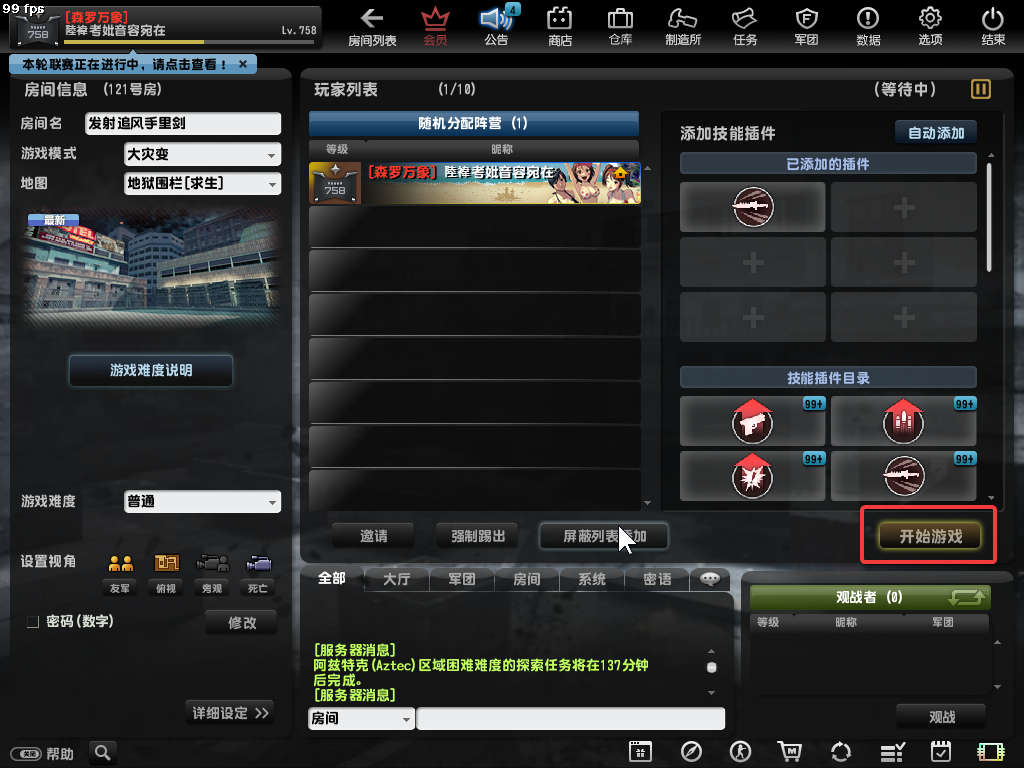
\includegraphics[width=\textwidth]{docs/assets/start_game.png}
    \caption{“开始游戏”按钮}
\end{figure}

\lstinline{CHOOSE_T_CLASS}:是否选择 T 阵营角色。如要选择 T 阵营角色,将其设置为 \lstinline{true},如要选择 CT 阵营角色,将其置为 \lstinline{false}。

\lstinline{CHOOSE_T_CLASS_X}、\lstinline{CHOOSE_T_CLASS_Y}:切换到 T 阵营选择界面的按钮坐标。

\begin{figure}[H]
    \Centering
    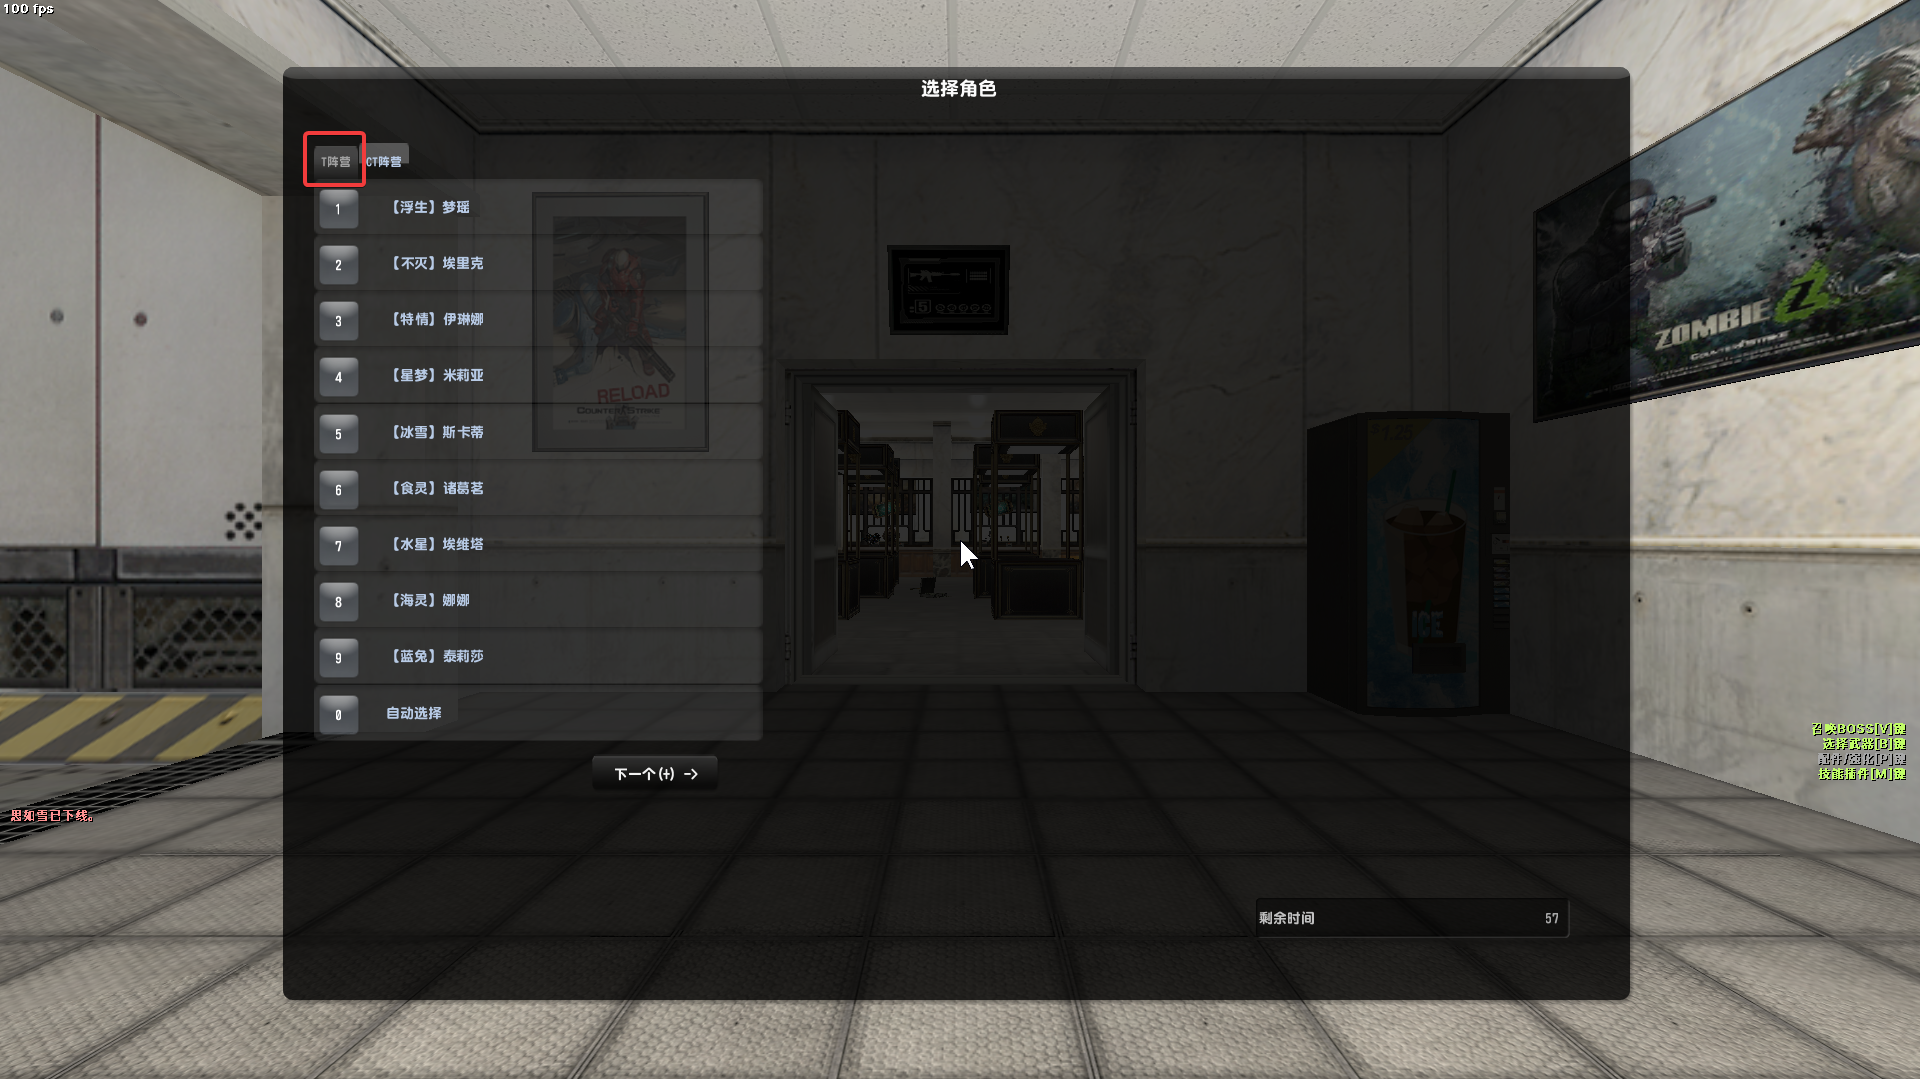
\includegraphics[width=\textwidth]{docs/assets/choose_T_class.png}
    \caption{“选择 T 阵营”按钮}
\end{figure}

\lstinline{CLASS_OPTION}:角色选项,取值范围为 0 ~ 9 的整数。

\lstinline{ZS_GAME_ESC_MENU_CANCEL_X}、\lstinline{ZS_GAME_ESC_MENU_CANCEL_Y}:“大灾变”模式下按 \lstinline{ESC} 后弹出的窗口中的“取消”按钮。
注意大灾变模式中取消按钮的位置与其他模式不同。

\begin{figure}[H]
    \Centering
    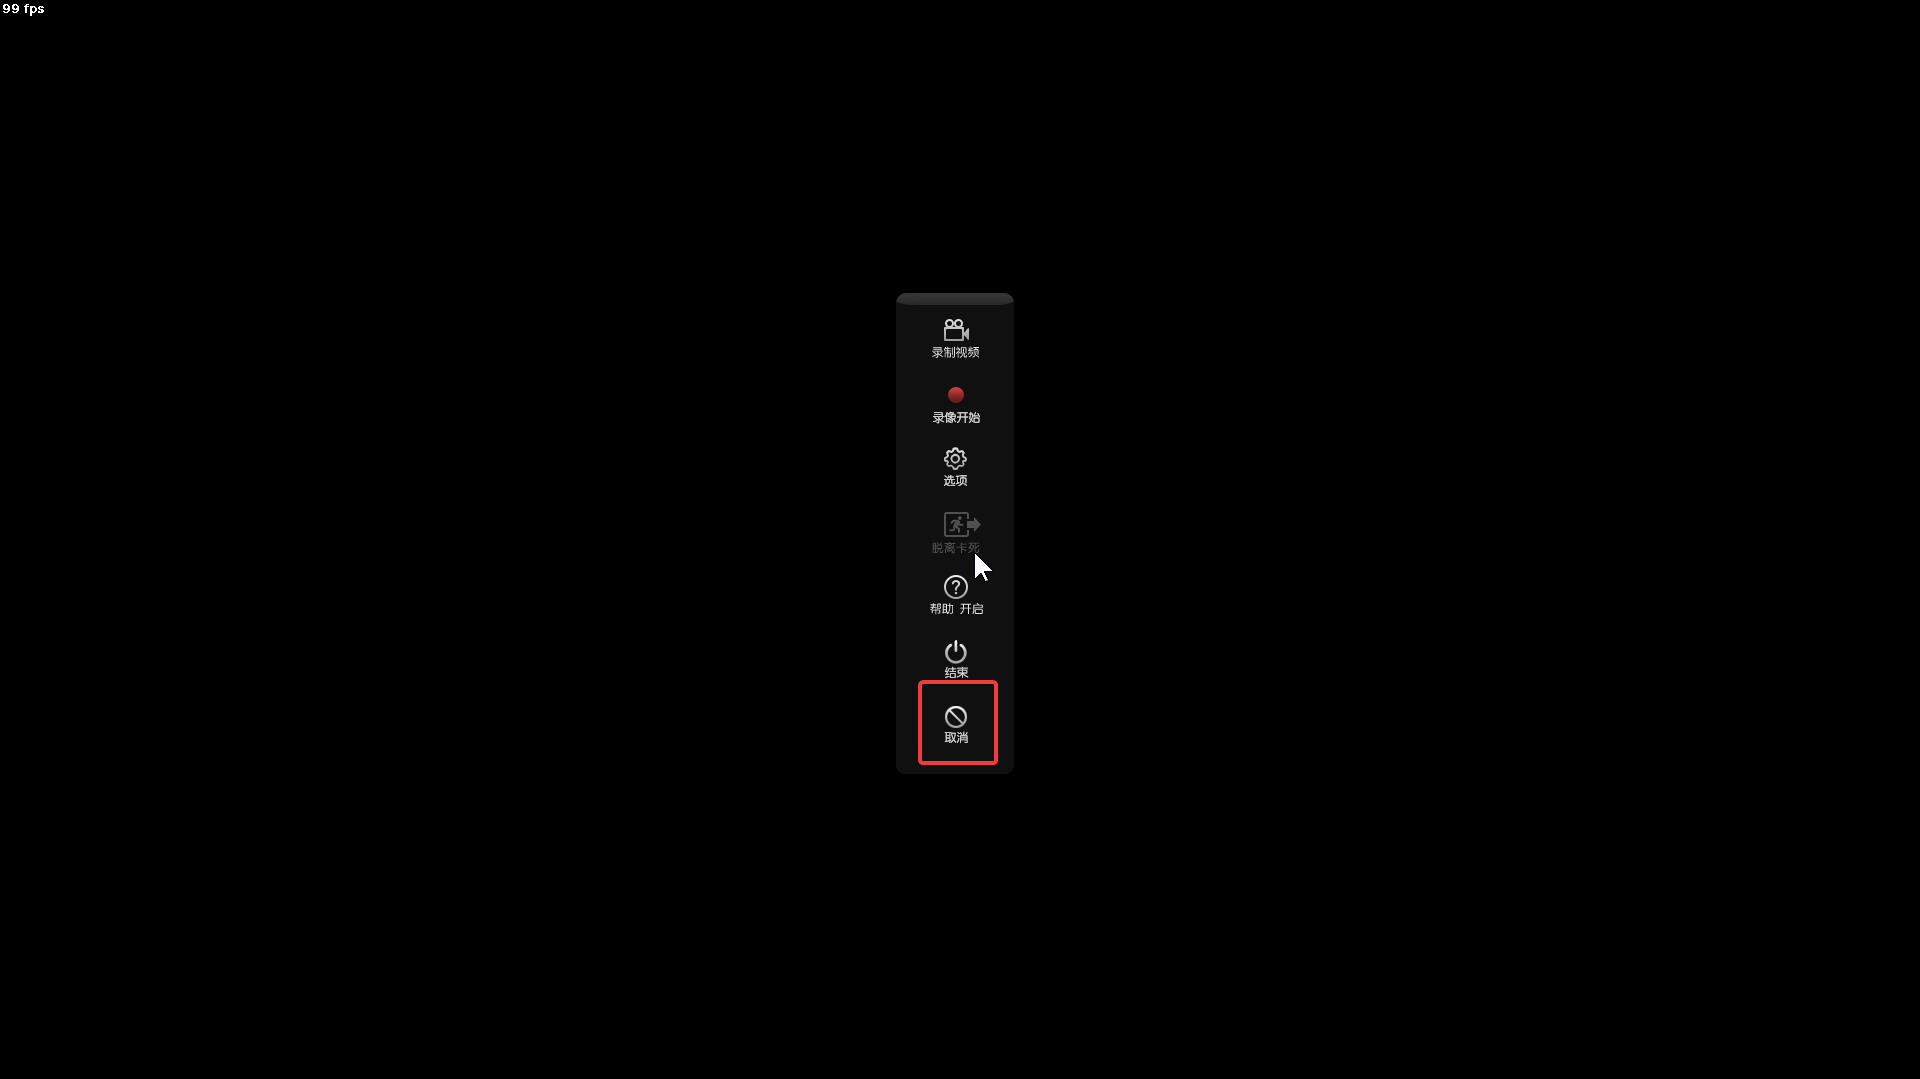
\includegraphics[width=\textwidth]{docs/assets/zs_esc_cancel.png}
    \caption{“大灾变”模式按下 \lstinline{ESC} 后的取消按钮}
\end{figure}

\lstinline{GAME_INSUFFICIENT_FUNDS_CONFIRM_X}、\lstinline{GAME_INSUFFICIENT_FUNDS_CONFIRM_Y}:“资金不足,无法购买”对话框中的“确认”按钮坐标。

\begin{figure}[H]
    \Centering
    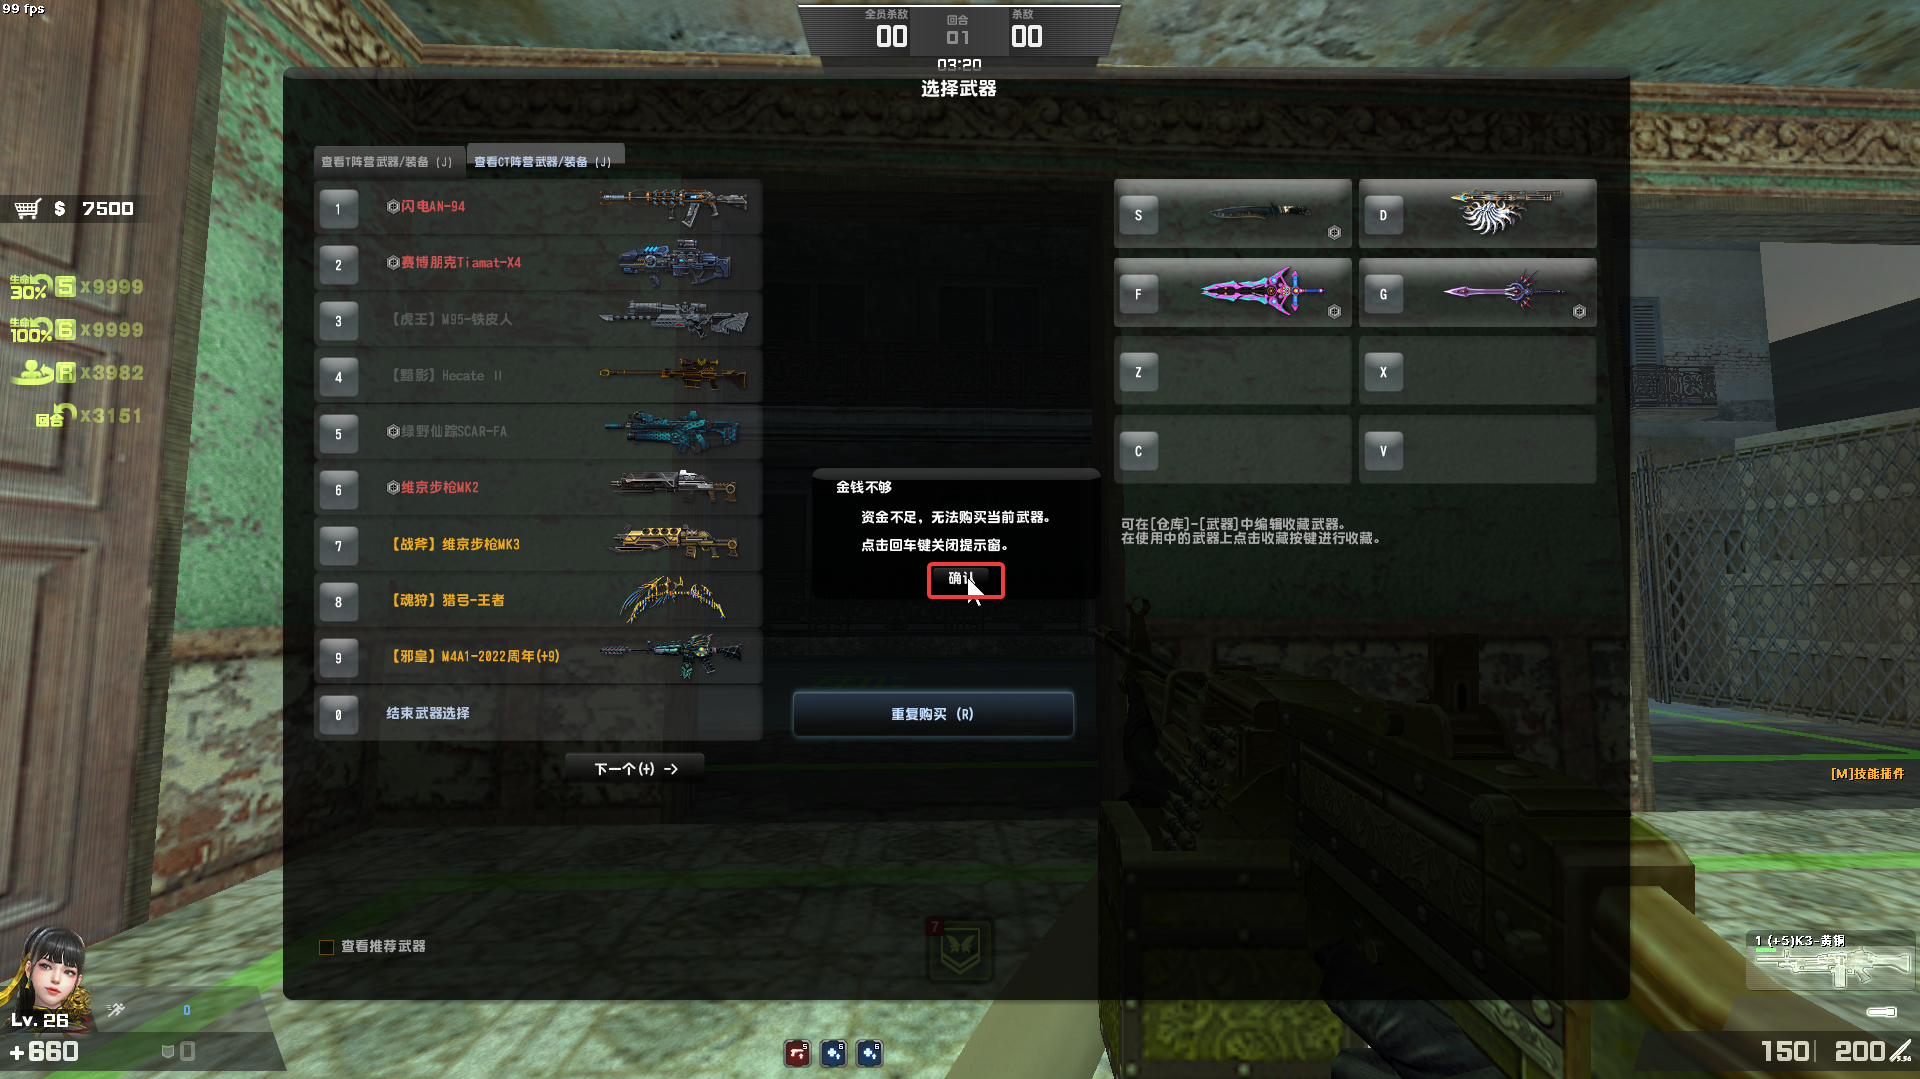
\includegraphics[width=\textwidth]{docs/assets/game_insuff_funds_confirm.png}
    \caption{“资金不足”确认按钮}
\end{figure}

\lstinline{GAME_DEAD_PURCHASE_MENU_REBUY_X}、\lstinline{GAME_DEAD_PURCHASE_MENU_REBUY_Y}:大灾变死亡后预购买菜单中的“重复购买”按钮。

\begin{figure}[H]
    \Centering
    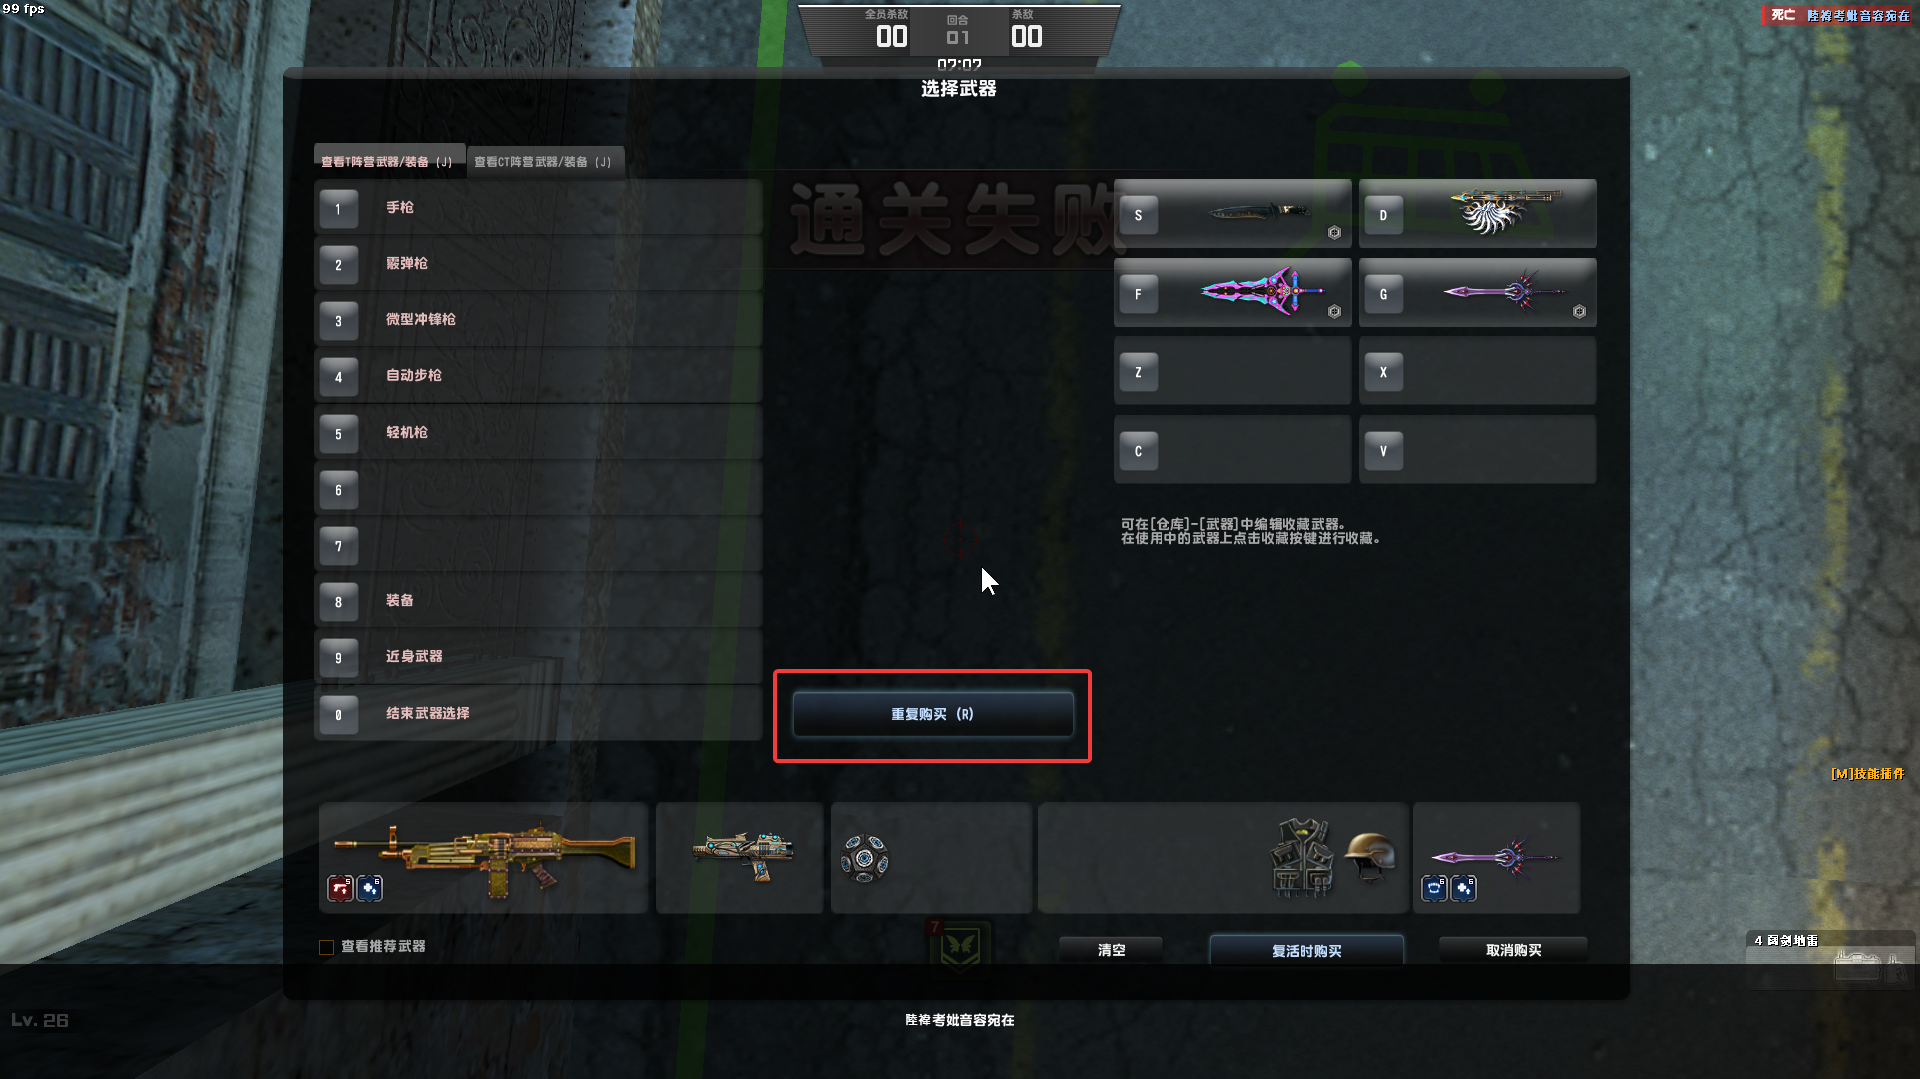
\includegraphics[width=\textwidth]{docs/assets/dead_purchase_rebuy.png}
    \caption{死亡时预购买界面中的“重复购买按钮”}
\end{figure}

\lstinline{GAME_ROUND_CONFIRM_X}、\lstinline{GAME_ROUND_CONFIRM_Y}:游戏结算界面的“确认”按钮坐标。

\begin{figure}[H]
    \Centering
    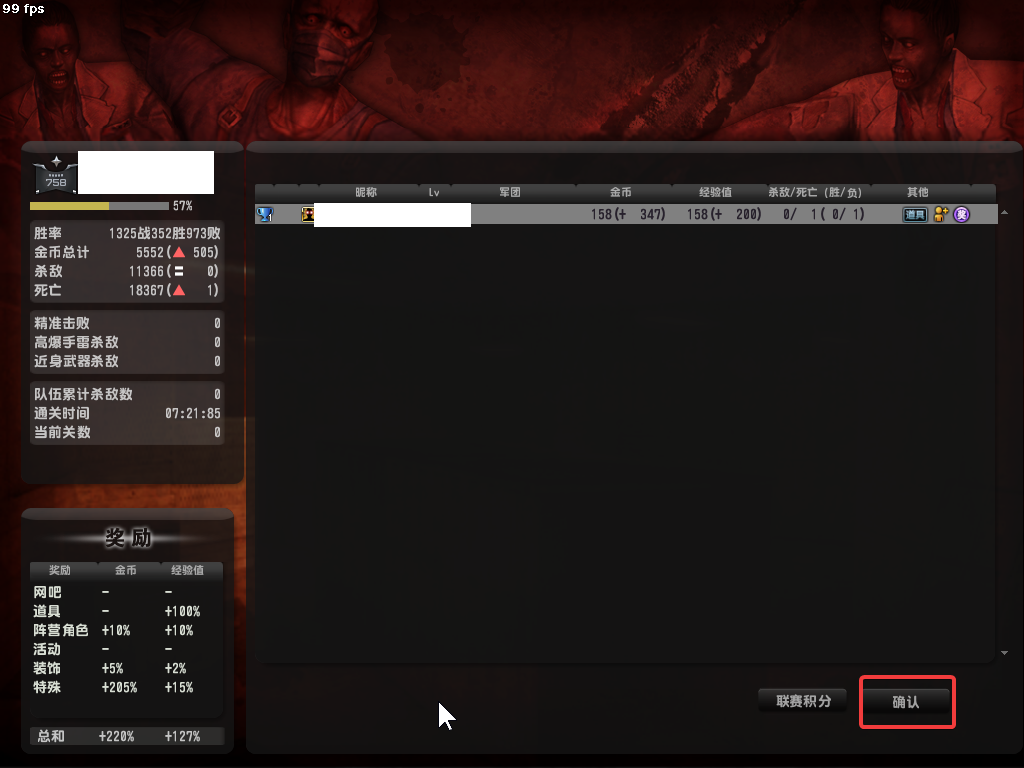
\includegraphics[width=\textwidth]{docs/assets/confirm_round.png}
    \caption{结算界面“确认”按钮}
\end{figure}

\subsubsection{配置购买武器列表}

打开 \lstinline{WeaponList.lua} 文件。文件中已经提供了大量样例,根据下述的说明仔细修改即可。

对于 1 号模式(单武器挂机,并购买配件武器),需要设置 \lstinline{PartWeaponList}(配件武器列表)和 \lstinline{DefaultWeaponList}(默认武器列表)。

配件武器列表格式如下(所有的标点符号\textbf{必须}为英文标点符号,下同):

\begin{minted}[breaklines, breakautoindent=true]{lua}
PartWeaponList = {
    Weapon:new({
        name = "星战前线·加特林",
        number = Weapon.PRIMARY,
        purchase_sequence = {Keyboard.B, Keyboard.J, Keyboard.TWO, Keyboard.FOUR}
    }),
    Weapon:new({
        name = "FNP-45战损版",
        number = Weapon.SECONDARY,
        purchase_sequence = {Keyboard.B, Keyboard.J, Keyboard.ONE, Keyboard.TWO}
    }),
        Weapon:new({
        name = "风暴之锤",
        number = Weapon.MELEE,
    }),
    Weapon:new({
        name = "燃爆Ignite-10",
        number = Weapon.GRENADE,
        purchase_sequence = {Keyboard.B, Keyboard.J, Keyboard.EIGHT, Keyboard.SEVEN}
    })
}
\end{minted}

每添加一款武器(数量任意,但鉴于配件武器不会被使用,故不建议超过 3 个),均需要在列表中新增相应的 \lstinline|Weapon:new({...})| 项。
\begin{itemize}

\item \lstinline{name} 为武器的名称,需要确保各个武器的名称彼此不同。

\item \lstinline{number} 为武器的序号,可以取:
\lstinline{Weapon.PRIMARY}(主武器)、\lstinline{Weapon.SECONDARY}(副武器)、\lstinline{Weapon.MELEE}(近战武器)、\lstinline{Weapon.GRENADE}(手雷)。

\item \lstinline{purchase_sequence}:武器购买按键序列。注意 \lstinline{Keyboard.J} 键可以切换不同阵营的武器。
对于暂时不需要的配件武器,例如上述的“风暴之锤”,可不设置 \lstinline{purchase_sequence},游戏中将不会购买。

\end{itemize}

默认武器列表虽不限制武器数量,但建议只设置一件武器,如\textbf{幻境!·光棱剑}。
除了\textbf{必须}设置 \lstinline{name}、\lstinline{number}、\lstinline{purchase_sequence} 外,还需要设置下列字段:

\begin{itemize}

\item \lstinline{switch_delay}(切枪延迟时间):整数,单位为毫秒,默认为 \lstinline{Delay.NORMAL}(100 毫秒)。

\item \lstinline{attack_button}(攻击鼠标按键):\lstinline{Mouse.LEFT}、\lstinline{Mouse.RIGHT}。

\end{itemize}

对于 2 号模式,需要设置 \lstinline{ExtendedWeaponList}(扩展武器列表,不限制武器数量,随机从中抽取武器并使用,器配置方式同 \lstinline{DefaultWeaponList})
和 \lstinline{SpecialWeapon}(特殊武器,如圣翼皓印或炽翼魔印)。在提供的 \lstinline{WeaponList.lua} 样例文件中,
已经编写好了使用的方式,如需使用,只需要将其中的 \lstinline{purchase_sequence} 修改为自己使用的购买按键序列即可。
如果没有圣翼皓印,则只需要删除 \lstinline{SpecialWeapon}。
对于有一定编程基础的玩家,可以自定义 \lstinline{SpecialWeapon},重写 \lstinline{use} 方法。
游戏过程中会通过调用 \lstinline{use} 方法使用该特殊武器。

\subsection{使用方法}

上述配置无误后,进入一个挂机房间,按 \lstinline{Ctrl} \lstinline{Alt} \lstinline{Shift} \lstinline{1} 或 \lstinline{Ctrl} \lstinline{Alt} \lstinline{Shift} \lstinline{2} 开始挂机。
对于模式 2,随机购买武器挂机功能将于 120 秒后有充足资金时启用。

在游戏因诸种原因掉线或闪退后,将自动尝试重启游戏,创建地狱围栏房间挂机。